\documentclass[]{article}
\usepackage{lmodern}
\usepackage{amssymb,amsmath}
\usepackage{ifxetex,ifluatex}
\usepackage{fixltx2e} % provides \textsubscript
\ifnum 0\ifxetex 1\fi\ifluatex 1\fi=0 % if pdftex
  \usepackage[T1]{fontenc}
  \usepackage[utf8]{inputenc}
\else % if luatex or xelatex
  \ifxetex
    \usepackage{mathspec}
  \else
    \usepackage{fontspec}
  \fi
  \defaultfontfeatures{Ligatures=TeX,Scale=MatchLowercase}
\fi
% use upquote if available, for straight quotes in verbatim environments
\IfFileExists{upquote.sty}{\usepackage{upquote}}{}
% use microtype if available
\IfFileExists{microtype.sty}{%
\usepackage{microtype}
\UseMicrotypeSet[protrusion]{basicmath} % disable protrusion for tt fonts
}{}
\usepackage[margin=1in]{geometry}
\usepackage{hyperref}
\hypersetup{unicode=true,
            pdftitle={Correlation analysis},
            pdfauthor={Matt Blanchard},
            pdfborder={0 0 0},
            breaklinks=true}
\urlstyle{same}  % don't use monospace font for urls
\usepackage{graphicx,grffile}
\makeatletter
\def\maxwidth{\ifdim\Gin@nat@width>\linewidth\linewidth\else\Gin@nat@width\fi}
\def\maxheight{\ifdim\Gin@nat@height>\textheight\textheight\else\Gin@nat@height\fi}
\makeatother
% Scale images if necessary, so that they will not overflow the page
% margins by default, and it is still possible to overwrite the defaults
% using explicit options in \includegraphics[width, height, ...]{}
\setkeys{Gin}{width=\maxwidth,height=\maxheight,keepaspectratio}
\IfFileExists{parskip.sty}{%
\usepackage{parskip}
}{% else
\setlength{\parindent}{0pt}
\setlength{\parskip}{6pt plus 2pt minus 1pt}
}
\setlength{\emergencystretch}{3em}  % prevent overfull lines
\providecommand{\tightlist}{%
  \setlength{\itemsep}{0pt}\setlength{\parskip}{0pt}}
\setcounter{secnumdepth}{0}
% Redefines (sub)paragraphs to behave more like sections
\ifx\paragraph\undefined\else
\let\oldparagraph\paragraph
\renewcommand{\paragraph}[1]{\oldparagraph{#1}\mbox{}}
\fi
\ifx\subparagraph\undefined\else
\let\oldsubparagraph\subparagraph
\renewcommand{\subparagraph}[1]{\oldsubparagraph{#1}\mbox{}}
\fi

%%% Use protect on footnotes to avoid problems with footnotes in titles
\let\rmarkdownfootnote\footnote%
\def\footnote{\protect\rmarkdownfootnote}

%%% Change title format to be more compact
\usepackage{titling}

% Create subtitle command for use in maketitle
\newcommand{\subtitle}[1]{
  \posttitle{
    \begin{center}\large#1\end{center}
    }
}

\setlength{\droptitle}{-2em}

  \title{Correlation analysis}
    \pretitle{\vspace{\droptitle}\centering\huge}
  \posttitle{\par}
    \author{Matt Blanchard}
    \preauthor{\centering\large\emph}
  \postauthor{\par}
      \predate{\centering\large\emph}
  \postdate{\par}
    \date{14/05/2019}


\begin{document}
\maketitle

\subsection{First, let's look at the relationship between accuracy
variables}\label{first-lets-look-at-the-relationship-between-accuracy-variables}

\begin{verbatim}
##              adr.ind.acc crt.ind.acc gk.ind.accO gk.ind.accR gk.ind.accUR mdmt.ind.acc rapm.ind.acc
## adr.grp.acc         0.89        0.42        0.35        0.31         0.23         0.35         0.44
## crt.grp.acc         0.53        0.89        0.21        0.23                      0.41         0.53
## gk.grp.accO                                 0.79        0.59         0.64                          
## gk.grp.accR                                 0.54        0.74                                       
## gk.grp.accUR                                 0.6                     0.77                          
## mdmt.grp.acc        0.38        0.34                                              0.48         0.39
## rapm.grp.acc        0.46        0.56                                              0.47         0.78
\end{verbatim}

Within the same test, we can see that individual and group accuracy
(diagonal in correlation matrix) is strongly and positively correlated
for all tests.

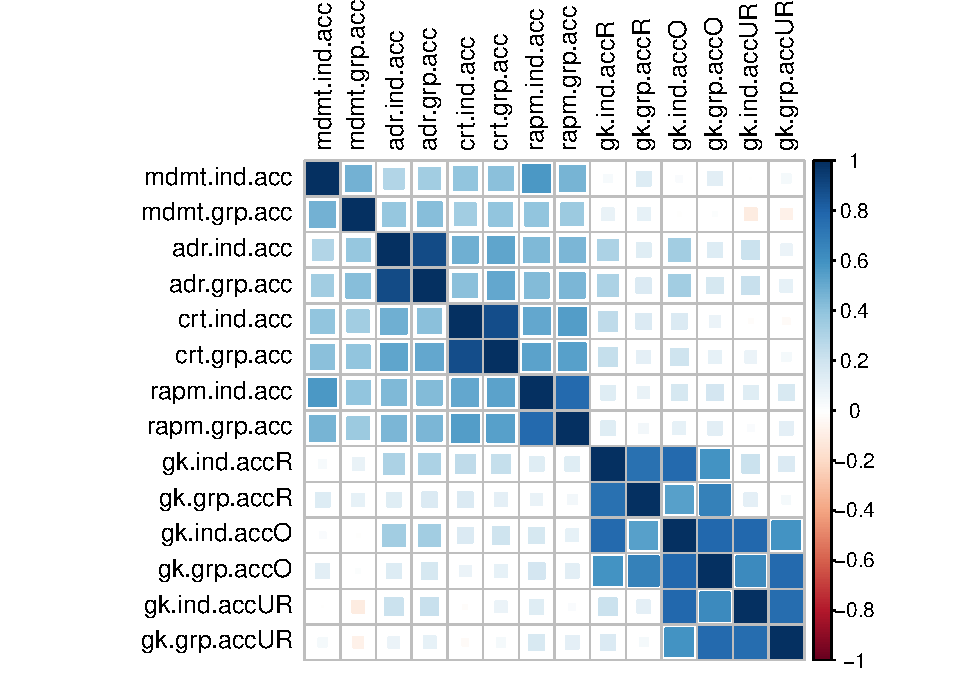
\includegraphics{corr_analyses_files/figure-latex/accuracy2-1.pdf}

\subsubsection{In the correlation plot two clusters are
evident:}\label{in-the-correlation-plot-two-clusters-are-evident}

\begin{itemize}
\tightlist
\item
  The cluster in the top left corner is a positive manifold between
  accuracy varaibles on ADR, CRT, MDMT and RAPM form. Individuals and
  dyads that perform well on one of these tests tend to perform well on
  the other tests.
\item
  The second cluster in the bottom right corner contains only the
  general-knowledge test accuracy varaibles. Performance on this test is
  not related to performance on the other tests.
\end{itemize}

\subsection{Next, let's check out the confidence
variables}\label{next-lets-check-out-the-confidence-variables}

\begin{verbatim}
##               adr.ind.conf crt.ind.conf gk.ind.confO gk.ind.confR gk.ind.confUR mdmt.ind.conf rapm.ind.conf
## adr.grp.conf          0.93         0.63         0.48         0.51          0.43          0.38          0.53
## crt.grp.conf          0.75         0.81         0.48         0.51          0.43          0.45          0.63
## gk.grp.confO          0.48         0.40         0.93         0.89          0.91          0.28          0.23
## gk.grp.confR          0.50         0.44         0.91         0.90          0.86          0.31          0.26
## gk.grp.confUR         0.44         0.33         0.90         0.84          0.92          0.23          0.19
## mdmt.grp.conf         0.59         0.49         0.37         0.39          0.33          0.57          0.55
## rapm.grp.conf         0.63         0.59         0.38         0.39          0.35          0.50          0.77
\end{verbatim}

Within the same test, we can see that individual and group confidence
(diagonal in correlation matrix) is strongly and positively correlated
for all tests.

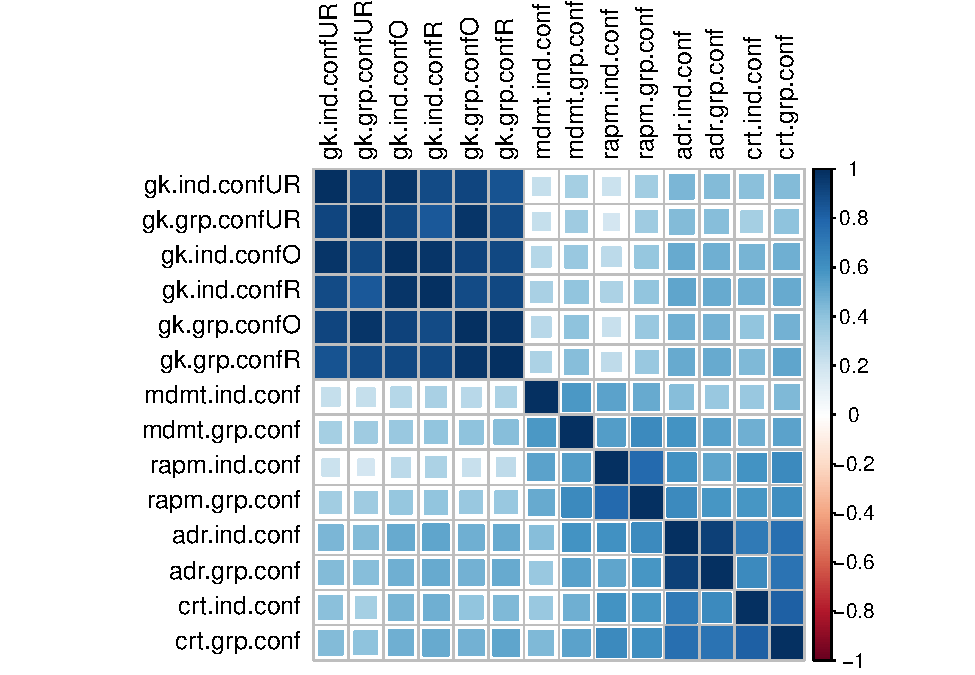
\includegraphics{corr_analyses_files/figure-latex/confidence2-1.pdf}

There is a positive manifold between all confidence variables.
Indicating that higher confidence on one test tends to be associated
with higher confidence on the other tests.

\subsection{Do accuracy and confidence
correlate?}\label{do-accuracy-and-confidence-correlate}

\begin{verbatim}
##               adr.ind.acc crt.ind.acc gk.ind.accO gk.ind.accR gk.ind.accUR mdmt.ind.acc rapm.ind.acc adr.grp.acc crt.grp.acc gk.grp.accO gk.grp.accR gk.grp.accUR mdmt.grp.acc rapm.grp.acc
## adr.ind.conf         0.38        0.45                                              0.29         0.28        0.39        0.45                                                           0.35
## crt.ind.conf         0.25        0.55                                              0.24         0.32        0.26        0.46                                                           0.36
## gk.ind.confO                                             0.22                                                                                                                              
## gk.ind.confR                                             0.25                                                                                                                              
## gk.ind.confUR                                                                                                                                                                              
## mdmt.ind.conf        0.23        0.37                                              0.71          0.4        0.29        0.34                                               0.3         0.41
## rapm.ind.conf        0.34         0.5                                               0.5         0.63        0.35         0.5                                              0.28         0.61
## adr.grp.conf         0.41        0.39        0.24                     0.21         0.23         0.24        0.45        0.39        0.21                                               0.32
## crt.grp.conf         0.37        0.61                                              0.34         0.44        0.38        0.61                                              0.23         0.42
## gk.grp.confO                                 0.21        0.23                                                                                                                              
## gk.grp.confR                                 0.23        0.28                                                                                                                              
## gk.grp.confUR                                                                                                                                                                              
## mdmt.grp.conf        0.22        0.36                                              0.36         0.36        0.29        0.36                                              0.38         0.36
## rapm.grp.conf        0.26        0.43                                              0.41         0.55        0.29         0.4                                              0.23         0.64
\end{verbatim}

Within the same test, we can see that accuracy and confidence (diagonal
in correlation matrix) is moderately and positively correlated for all
tests except GK.

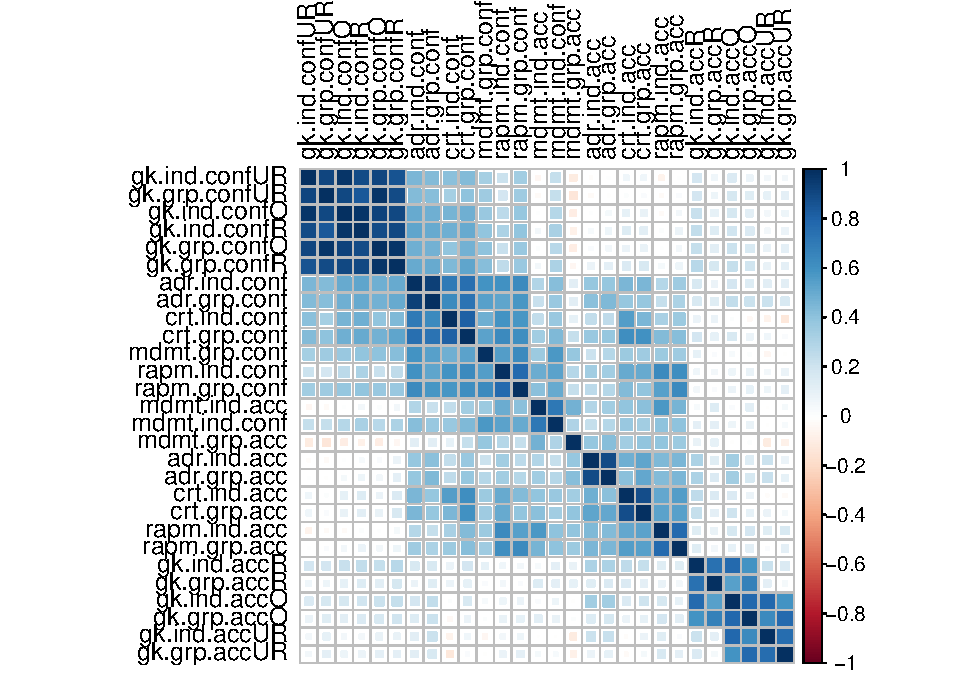
\includegraphics{corr_analyses_files/figure-latex/acc-conf2-1.pdf}

There is a positive manifold between all accuracy and confidence
variables except the general-knowledge test. Indicating that
participants with higher confidence tend to have higher accuracy on all
tests except GK.

\subsection{What about the POST
variables?}\label{what-about-the-post-variables}

\begin{verbatim}
##               adr.ind.post crt.ind.post gk.ind.postO gk.ind.postR gk.ind.postUR mdmt.ind.post rapm.ind.post
## adr.grp.post          0.64         0.35         0.41         0.27          0.38                         0.2
## crt.grp.post          0.31          0.4          0.5         0.46          0.36                        0.45
## gk.grp.postO                                    0.62         0.49          0.43          0.25          0.32
## gk.grp.postR          0.38                      0.66         0.63          0.52                         0.4
## gk.grp.postUR                                   0.47         0.36          0.42          0.32              
## mdmt.grp.post                                                                                              
## rapm.grp.post         0.42         0.22         0.46         0.42          0.39                        0.48
\end{verbatim}

Within the same test, we can see that individual and group POSTs
(diagonal in correlation matrix) are moderately and positively
correlated for all tests except MDMT.

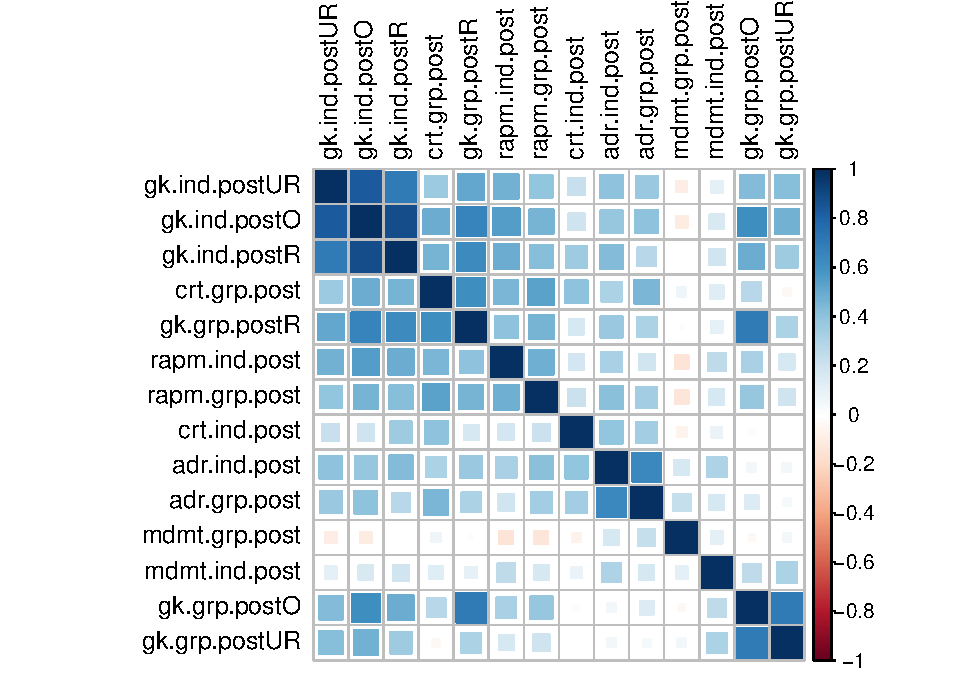
\includegraphics{corr_analyses_files/figure-latex/post2-1.pdf}

With the exception of MDMT, there appears to be a positive manifold
between POST variables. Indicating that higher POST scores on one test
tend to be associated with higher POST scores on the other tests.

\subsection{How does POST relate to accuracy and
confidence?}\label{how-does-post-relate-to-accuracy-and-confidence}

\begin{verbatim}
##               adr.ind.post crt.ind.post gk.ind.postO gk.ind.postR gk.ind.postUR mdmt.ind.post rapm.ind.post adr.grp.post crt.grp.post gk.grp.postO gk.grp.postR gk.grp.postUR mdmt.grp.post rapm.grp.post
## adr.ind.acc                                                                                                                                                                                              
## crt.ind.acc                         0.2                                                                                                                                                                  
## gk.ind.accO                                                                                                                                                                            0.45              
## gk.ind.accR                                                                                                                                                                             0.2              
## gk.ind.accUR                                    0.21                        0.2                                                                                                        0.52              
## mdmt.ind.acc                                                                                            0.2                                                                                              
## rapm.ind.acc                                                                                                                                                             0.22                            
## adr.grp.acc                                                                                                                                                                                              
## crt.grp.acc                                                                                                                                                                                              
## gk.grp.accO           0.23                                                                                                                                                             0.44              
## gk.grp.accR                                                                                                                                                                                              
## gk.grp.accUR          0.25                                                                                                                                                             0.55              
## mdmt.grp.acc                                                              -0.24                                                                                                                          
## rapm.grp.acc          0.25                                                                              0.2                                    0.2                       0.25                            
## adr.ind.conf          0.45         0.25                      0.23                                      0.31         0.44         0.27                      0.31                         0.2              
## crt.ind.conf          0.24         0.31                                                   0.2          0.24                      0.23                      0.28                                          
## gk.ind.confO          0.29                                                 0.28                                                  0.23                      0.28                                      0.21
## gk.ind.confR          0.28                                                 0.23                                                                            0.23                        0.24              
## gk.ind.confUR         0.28                                   0.21          0.31                                                  0.28                      0.32                                      0.23
## mdmt.ind.conf         0.27                                                               0.46          0.31                                                 0.2          0.31          0.32              
## rapm.ind.conf         0.38                                                               0.22          0.38                                                0.22          0.26          0.23              
## adr.grp.conf          0.39         0.21                       0.2                                      0.27         0.54         0.34                      0.35                        0.33              
## crt.grp.conf          0.28          0.2                                                                0.25         0.21         0.43                      0.31                        0.29              
## gk.grp.confO          0.32                                                 0.21                                                   0.2                      0.25                        0.32              
## gk.grp.confR          0.32                                                                                                        0.2                      0.24                        0.36              
## gk.grp.confUR          0.3                                                 0.27                                                                            0.24          0.21          0.26              
## mdmt.grp.conf         0.34                                                               0.36                                                 0.21          0.2          0.31          0.51              
## rapm.grp.conf         0.38                                                 0.22          0.27          0.23         0.24                                   0.21          0.27          0.45           0.2
\end{verbatim}

Within the same test, we can see that individual and group POSTs
(diagonal in correlation matrix) are moderately and positively
correlated with confidence for all tests except GK individual responses.
There is no relationship between POST and accuracy.

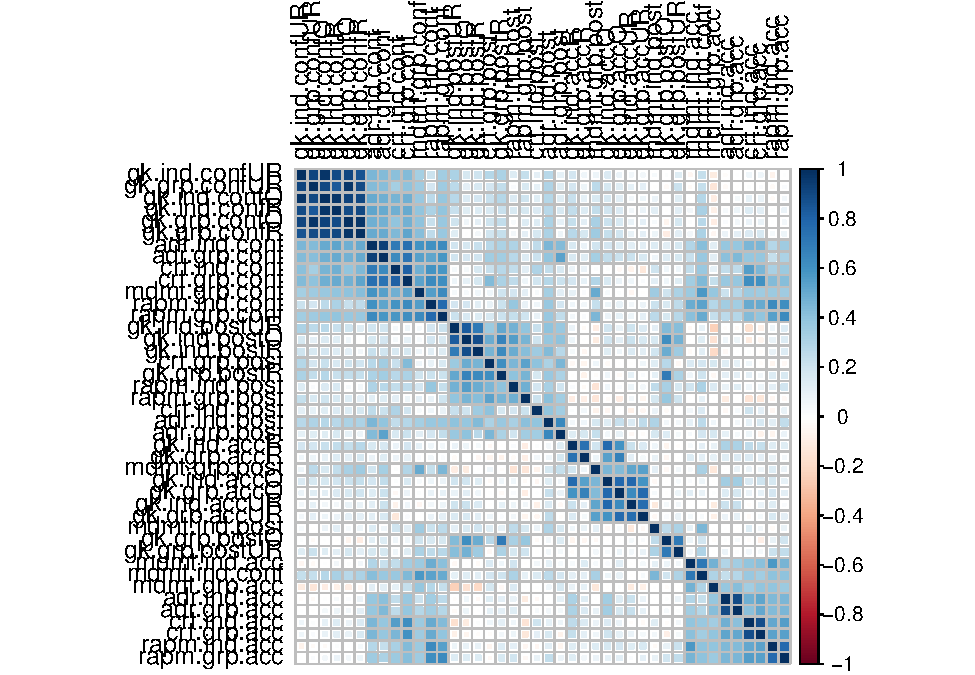
\includegraphics{corr_analyses_files/figure-latex/post4-1.pdf}

A number of clusters have formed: * confidence variables (top left) *
POST variables (along the diagonal below the confidence cluster) * a
weaker cluster containing confidence and POST varibles * GK accuracy
(along the diagonal below the POST cluster) * accuracy on the other
tests (along the diagonal below the GK accuracy cluster)

\subsection{Let's take a look at the DPA
variables}\label{lets-take-a-look-at-the-dpa-variables}

\subsubsection{Decisiveness}\label{decisiveness}

\begin{verbatim}
##              adr.ind.dec crt.ind.dec gk.ind.decO gk.ind.decR gk.ind.decUR mdmt.ind.dec rapm.ind.dec
## adr.grp.dec         0.75        0.52        0.43        0.43          0.4                          
## crt.grp.dec          0.6        0.74        0.36        0.34         0.37                       0.4
## gk.grp.decO          0.5        0.48        0.88        0.83         0.86                          
## gk.grp.decR         0.49        0.48        0.84        0.83          0.8                          
## gk.grp.decUR        0.47        0.44        0.84        0.77         0.85                          
## mdmt.grp.dec                                                                      0.31             
## rapm.grp.dec        0.55        0.55        0.38        0.37         0.35         0.32         0.56
\end{verbatim}

Within the same test, we can see that individual and group decisiveness
(diagonal in correlation matrix) are moderately and positively
correlated for all tests.

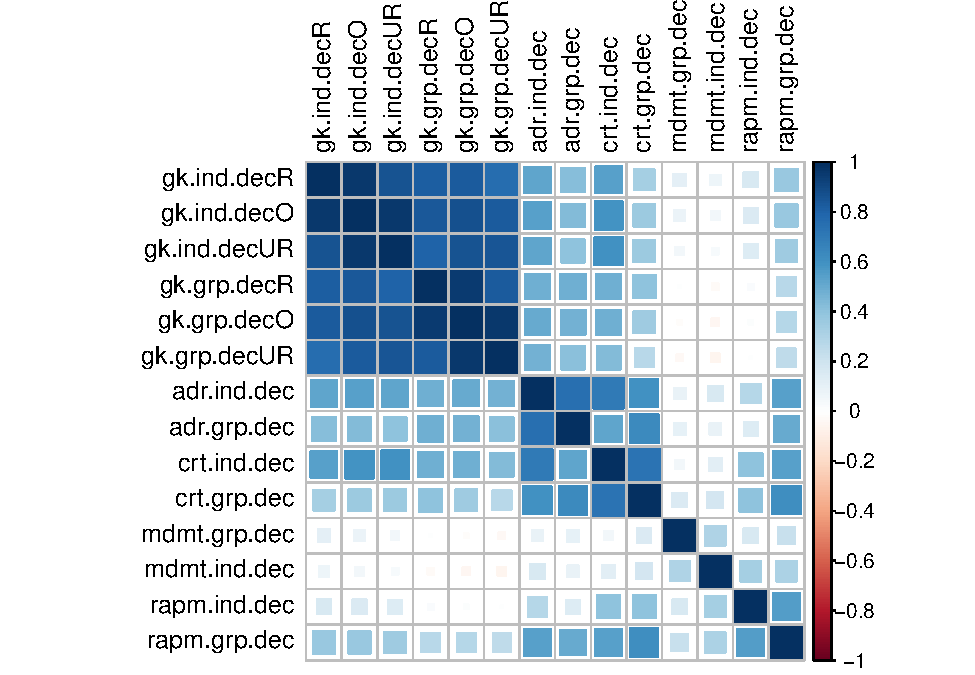
\includegraphics{corr_analyses_files/figure-latex/decisiveness2-1.pdf}

With the exception of MDMT, there appears to be a positive manifold
between the decisiveness variables. It is worth noting that RAPM
correlates more weakly with GK tests. This pattern indicates that higher
decisiveness on one test tends to be associated with higher decisiveness
scores on the other tests.

\subsubsection{Recklessness}\label{recklessness}

\begin{verbatim}
##              adr.ind.rec crt.ind.rec gk.ind.recO gk.ind.recR gk.ind.recUR mdmt.ind.rec rapm.ind.rec
## adr.grp.rec          0.6         0.3        0.26        0.27                                       
## crt.grp.rec         0.44        0.49        0.30        0.34         0.21                          
## gk.grp.recO         0.35        0.42        0.79        0.73         0.71                          
## gk.grp.recR         0.29        0.34        0.67        0.69         0.57                          
## gk.grp.recUR        0.31        0.42        0.73        0.64         0.68                          
## mdmt.grp.rec                               -0.20                    -0.22                          
## rapm.grp.rec                    0.21        0.22        0.22
\end{verbatim}

Within the same test, we can see that individual and group recklessness
(diagonal in correlation matrix) are moderately and positively
correlated for ADR, CRT and GK but not for MDMT or RAPM.

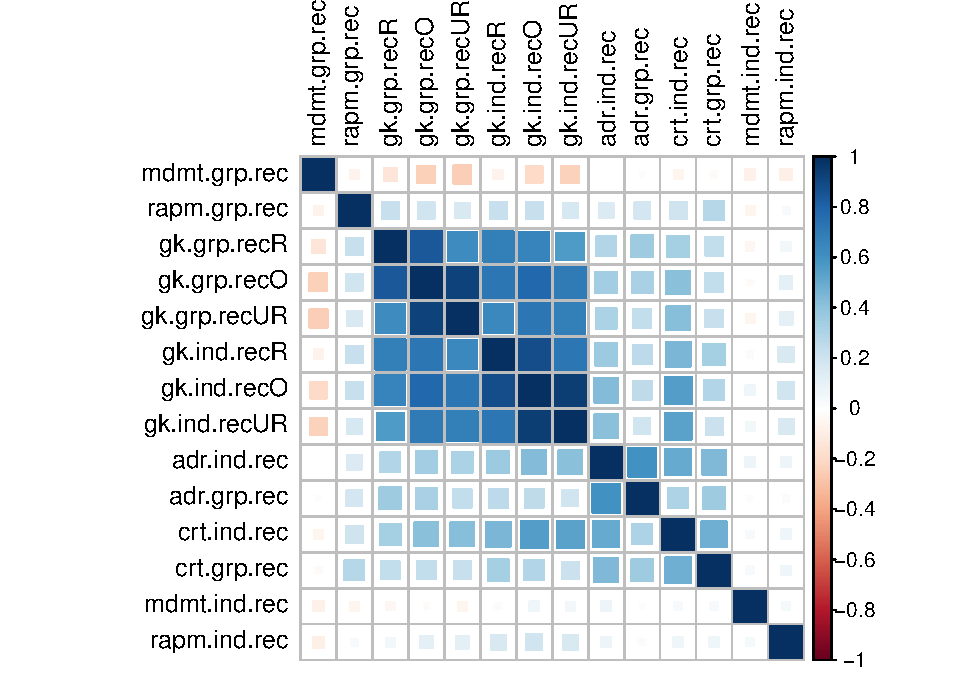
\includegraphics{corr_analyses_files/figure-latex/recklessness2-1.pdf}

There is a positive manifold between the recklessness variables for ADR,
CRT and GK. This pattern indicates that higher recklessness on one of
these tests tends to be associated with higher recklessness scores on
the other tests. Recklessness on MDMT and RAPM does not correlate
significantly with any of the other tests or each other.

\subsubsection{Optimality}\label{optimality}

\begin{verbatim}
##                adr.ind.optim crt.ind.optim gk.ind.optimO gk.ind.optimR gk.ind.optimUR mdmt.ind.optim rapm.ind.optim
## adr.grp.optim           0.85           0.5          0.31          0.29           0.29           0.36           0.37
## crt.grp.optim           0.59          0.87          0.29          0.23           0.31           0.39           0.56
## gk.grp.optimO           0.29          0.25          0.85          0.76           0.81                              
## gk.grp.optimR           0.27          0.31          0.82          0.82           0.69                              
## gk.grp.optimUR          0.26                         0.7          0.55           0.77                              
## mdmt.grp.optim          0.40          0.34                                                      0.45           0.35
## rapm.grp.optim          0.54          0.59          0.31          0.28            0.3           0.46           0.71
\end{verbatim}

Within the same test, we can see that individual and group optimality
(diagonal in correlation matrix) are strongly and positively correlated
for all tests.

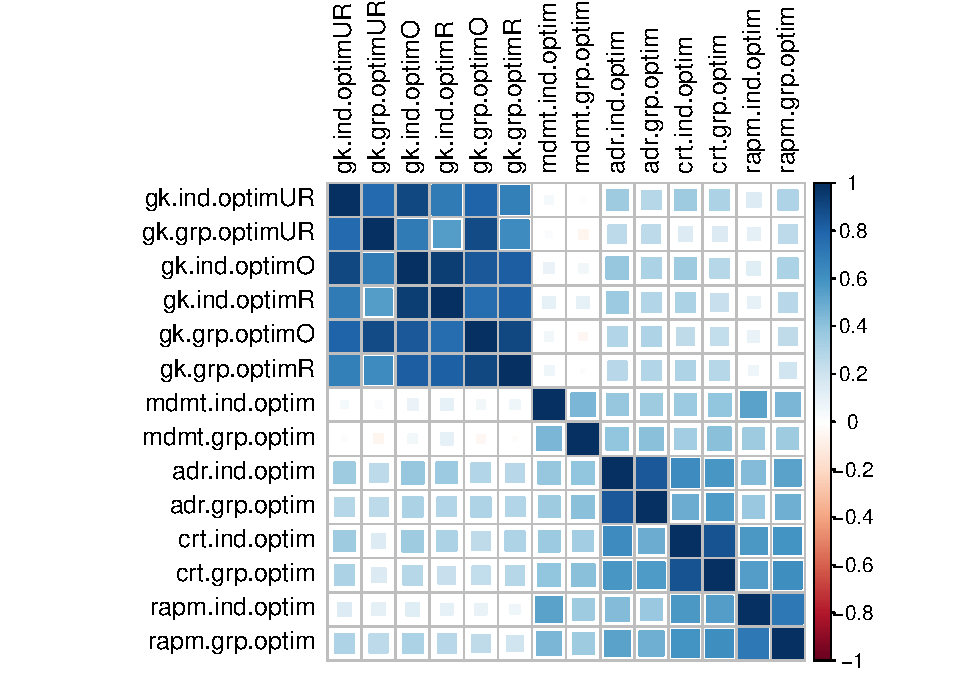
\includegraphics{corr_analyses_files/figure-latex/optimality2-1.pdf}

There is a positive manifold between the optimality variables. With two
caveats: 1) optimality on MDMT does not relate with GK and 2) ADR, CRT,
RAPM correltates strongly with each other but weakly (and significantly)
with GK. This pattern indicates that higher optimality on one test tends
to be associated with higher optimality on the other tests.

\subsubsection{Competence}\label{competence}

\begin{verbatim}
##               adr.ind.comp crt.ind.comp gk.ind.compO gk.ind.compR gk.ind.compUR mdmt.ind.comp rapm.ind.comp
## adr.grp.comp           0.7         0.39         0.25                       0.26          0.26              
## crt.grp.comp          0.48         0.57                                    0.22          0.25          0.23
## gk.grp.compO           0.2                      0.52         0.38          0.38                            
## gk.grp.compR                                    0.48         0.53                                          
## gk.grp.compUR                                   0.34                       0.42                            
## mdmt.grp.comp         0.34         0.24                                                                    
## rapm.grp.comp         0.34         0.23         0.34          0.3                        0.32          0.43
\end{verbatim}

Within the same test, we can see that individual and group competence
(diagonal in correlation matrix) is moderately and positively correlated
for all tests.

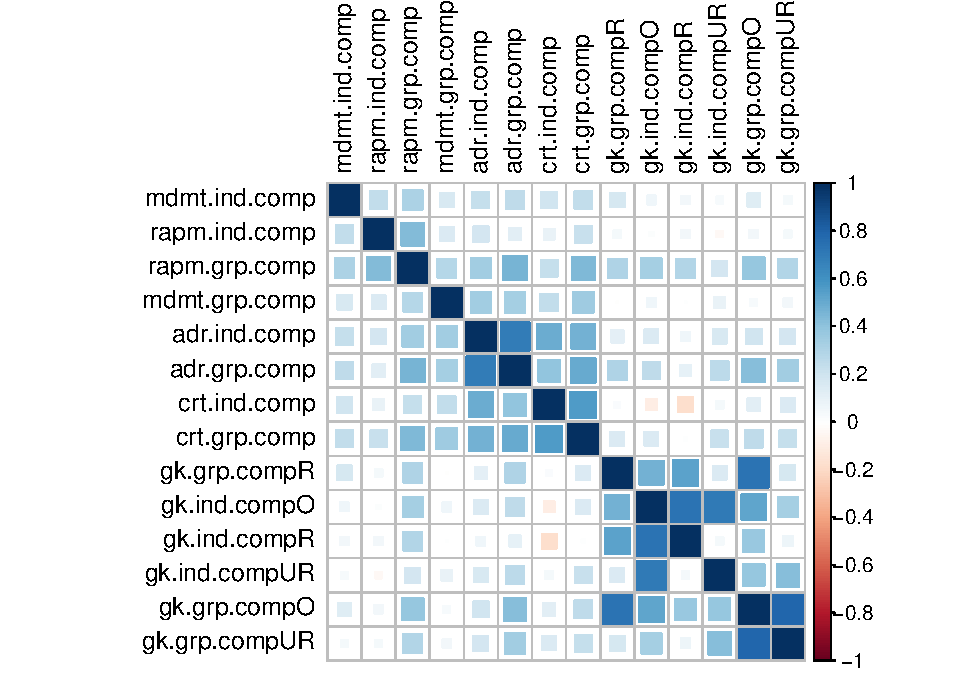
\includegraphics{corr_analyses_files/figure-latex/competence2-1.pdf}

There is a positive manifold between the optimality variables. With two
caveats: 1) optimality on MDMT does not relate with GK and 2) ADR, CRT,
RAPM correltates strongly with each other but weakly (and significantly)
with GK. This pattern indicates that higher optimality on one test tends
to be associated with higher optimality on the other tests.

\subsubsection{Hesitancy}\label{hesitancy}

\begin{verbatim}
##              adr.ind.hes crt.ind.hes gk.ind.hesO gk.ind.hesR gk.ind.hesUR mdmt.ind.hes rapm.ind.hes
## adr.grp.hes         0.65        0.29        0.45        0.44         0.42                      0.23
## crt.grp.hes         0.41        0.47        0.27        0.22         0.26         0.22         0.35
## gk.grp.hesO         0.43        0.29        0.82        0.76         0.78                          
## gk.grp.hesR         0.41        0.25        0.76        0.74         0.69                          
## gk.grp.hesUR         0.4         0.3        0.74        0.65         0.75                          
## mdmt.grp.hes                                                                      0.22             
## rapm.grp.hes        0.54        0.36        0.44        0.39         0.45          0.2         0.45
\end{verbatim}

Within the same test, we can see that individual and group hesitancy
(diagonal in correlation matrix) is moderately and positively correlated
for all tests.

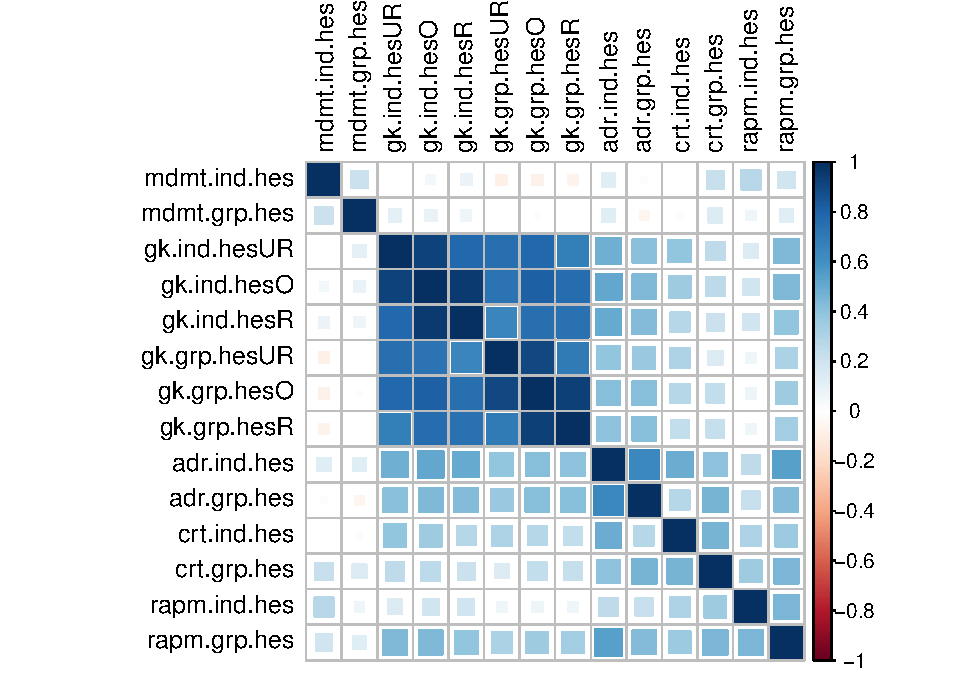
\includegraphics{corr_analyses_files/figure-latex/hesitancy2-1.pdf}

There is a positive manifold between the hesitancy variables with a
caveat: hesitancy on MDMT weakly relates to hesitancy on RAPM and CRT
but nothing else. This pattern indicates that higher hesitancy on one
test tends to be associated with higher hesitancy on the other tests.

\section{Now let's take a look at the relationships between our test
variables and
demographics}\label{now-lets-take-a-look-at-the-relationships-between-our-test-variables-and-demographics}

\subsection{Proportion of females and accuracy, confidence and
POST}\label{proportion-of-females-and-accuracy-confidence-and-post}

\begin{verbatim}
##               prop.female
## gk.ind.confR        -0.44
## gk.ind.confO        -0.43
## gk.grp.confR        -0.40
## gk.ind.confUR       -0.40
## crt.ind.conf        -0.38
## crt.grp.conf        -0.36
## gk.grp.confO        -0.36
## adr.ind.conf        -0.30
## crt.grp.acc         -0.30
## gk.grp.confUR       -0.29
## crt.ind.acc         -0.29
## mdmt.ind.conf       -0.28
## crt.grp.post        -0.28
## adr.grp.conf        -0.27
## rapm.grp.conf       -0.24
## gk.ind.accR         -0.22
## crt.ind.post        -0.22
## mdmt.grp.conf       -0.20
## mdmt.ind.post       -0.20
## rapm.ind.conf       -0.20
## adr.ind.acc         -0.17
## adr.grp.acc         -0.15
## gk.grp.postR        -0.14
## rapm.grp.acc        -0.13
## gk.grp.accR         -0.11
## mdmt.ind.acc        -0.10
## gk.ind.accO         -0.09
## mdmt.grp.post       -0.09
## mdmt.grp.acc        -0.08
## gk.grp.postUR       -0.08
## rapm.ind.post       -0.08
## gk.ind.accUR         0.07
## rapm.ind.acc        -0.04
## adr.ind.post        -0.04
## gk.grp.accUR         0.04
## gk.grp.accO         -0.04
## gk.grp.postO        -0.02
## adr.grp.post        -0.02
## gk.ind.postUR       -0.01
## gk.ind.postO        -0.01
## gk.ind.postR         0.01
## rapm.grp.post        0.00
\end{verbatim}

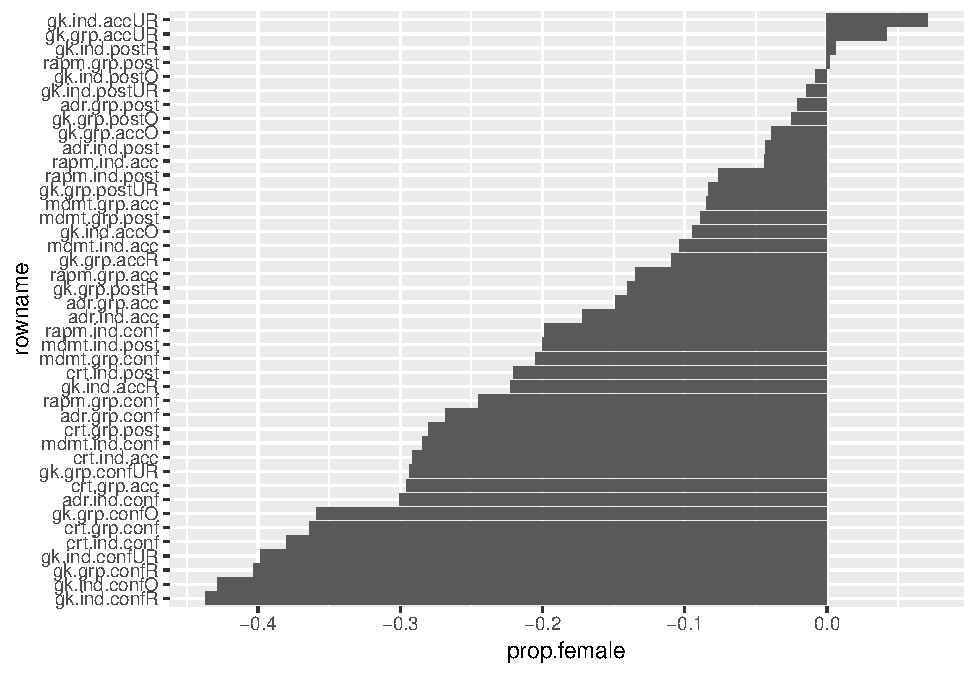
\includegraphics{corr_analyses_files/figure-latex/female1-1.pdf}

There is a consistent pattern of small to moderate significant negative
correlations between the confidence variables and the proportion of
females in a group. For CRT, accuracy and POST are also significantly
negatively correlated with the proportion of females.

\begin{verbatim}
##                prop.female
## adr.ind.dec          -0.26
## crt.ind.dec          -0.36
## gk.ind.decO          -0.40
## gk.ind.decR          -0.40
## gk.ind.decUR         -0.38
## mdmt.ind.dec         -0.17
## rapm.ind.dec         -0.10
## adr.grp.dec          -0.20
## crt.grp.dec          -0.22
## gk.grp.decO          -0.32
## gk.grp.decR          -0.33
## gk.grp.decUR         -0.29
## mdmt.grp.dec         -0.04
## rapm.grp.dec         -0.25
## adr.ind.rec          -0.11
## crt.ind.rec          -0.29
## gk.ind.recO          -0.34
## gk.ind.recR          -0.28
## gk.ind.recUR         -0.33
## mdmt.ind.rec         -0.30
## rapm.ind.rec         -0.03
## adr.grp.rec          -0.06
## crt.grp.rec          -0.06
## gk.grp.recO          -0.20
## gk.grp.recR          -0.14
## gk.grp.recUR         -0.18
## mdmt.grp.rec          0.05
## rapm.grp.rec         -0.06
## adr.ind.optim        -0.29
## crt.ind.optim        -0.37
## gk.ind.optimO        -0.42
## gk.ind.optimR        -0.43
## gk.ind.optimUR       -0.33
## mdmt.ind.optim       -0.12
## rapm.ind.optim       -0.08
## adr.grp.optim        -0.20
## crt.grp.optim        -0.30
## gk.grp.optimO        -0.27
## gk.grp.optimR        -0.33
## gk.grp.optimUR       -0.16
## mdmt.grp.optim       -0.10
## rapm.grp.optim       -0.24
## adr.ind.comp         -0.22
## crt.ind.comp         -0.11
## gk.ind.compO         -0.28
## gk.ind.compR         -0.31
## gk.ind.compUR        -0.09
## mdmt.ind.comp         0.02
## rapm.ind.comp        -0.05
## adr.grp.comp         -0.15
## crt.grp.comp         -0.21
## gk.grp.compO         -0.10
## gk.grp.compR         -0.24
## gk.grp.compUR         0.06
## mdmt.grp.comp        -0.11
## rapm.grp.comp        -0.23
## adr.ind.hes           0.29
## crt.ind.hes           0.27
## gk.ind.hesO           0.43
## gk.ind.hesR           0.42
## gk.ind.hesUR          0.38
## mdmt.ind.hes          0.10
## rapm.ind.hes          0.05
## adr.grp.hes           0.19
## crt.grp.hes           0.19
## gk.grp.hesO           0.35
## gk.grp.hesR           0.34
## gk.grp.hesUR          0.28
## mdmt.grp.hes          0.09
## rapm.grp.hes          0.23
\end{verbatim}

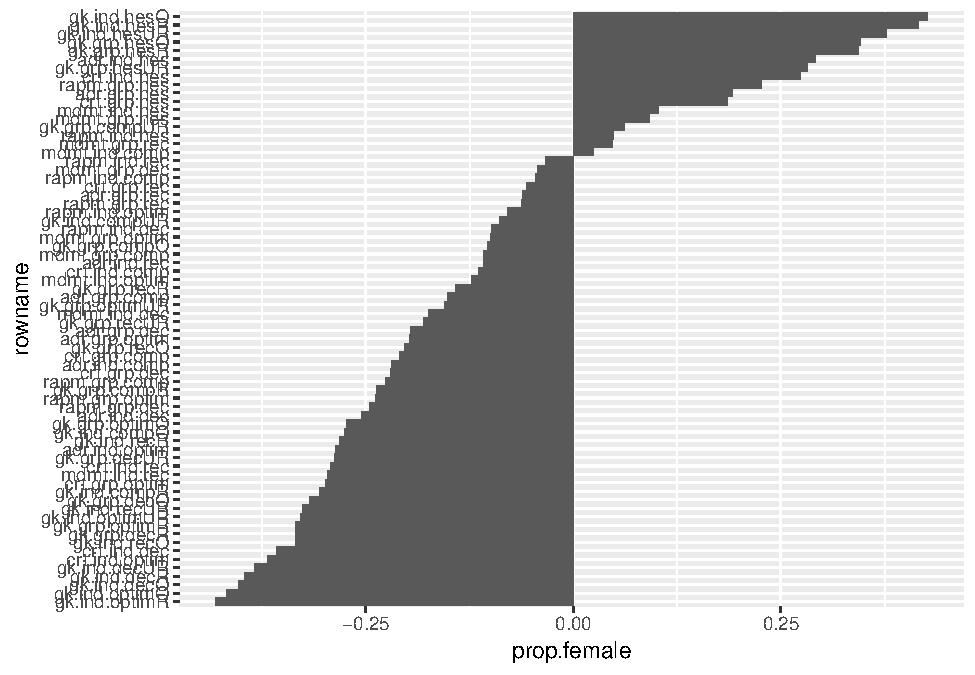
\includegraphics{corr_analyses_files/figure-latex/female2-1.pdf}

There is a consistent pattern of small to moderate significant positive
correlations between the hesitancy variables and the proportion of
females in a group. There is also a consistent pattern of small to
moderate significant negative correlations between the decisiveness and
optimality variables and the proportion of females. Correlations with
recklessness and competence are mixed.

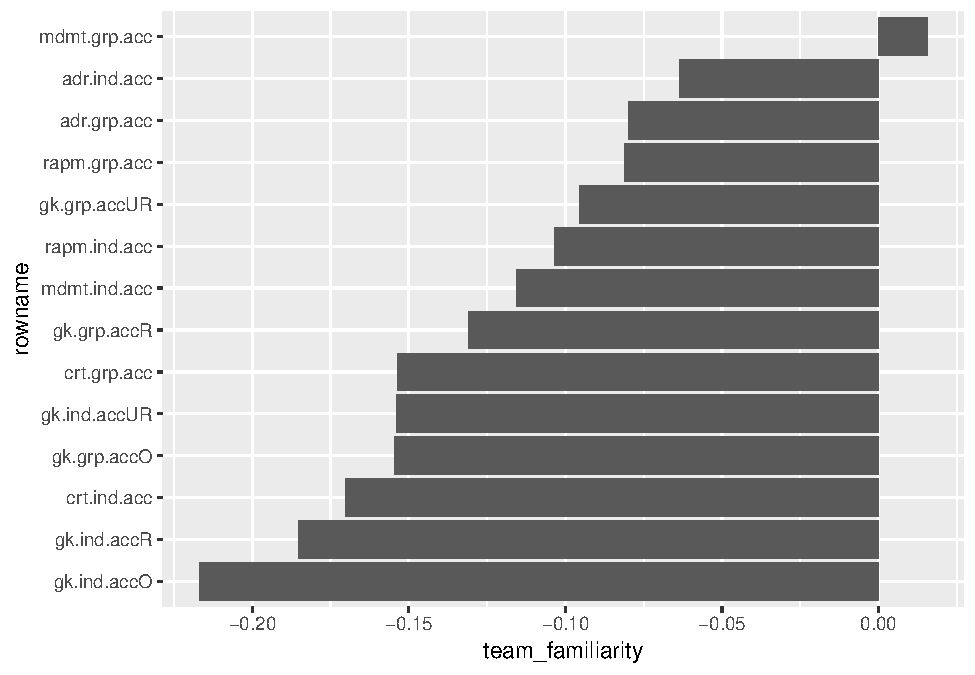
\includegraphics{corr_analyses_files/figure-latex/unnamed-chunk-1-1.pdf}
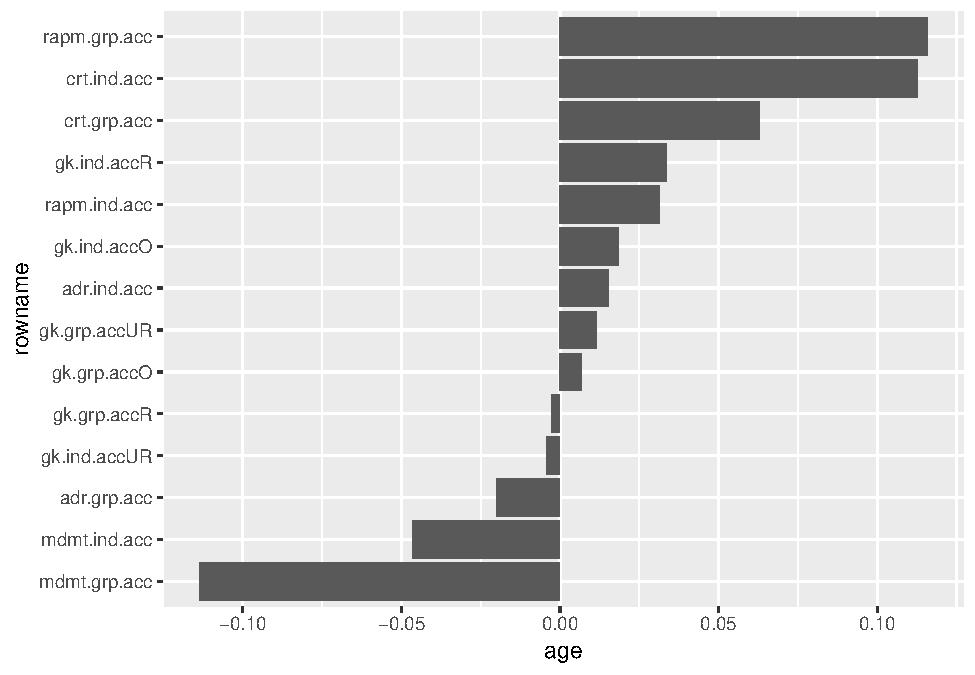
\includegraphics{corr_analyses_files/figure-latex/unnamed-chunk-1-2.pdf}
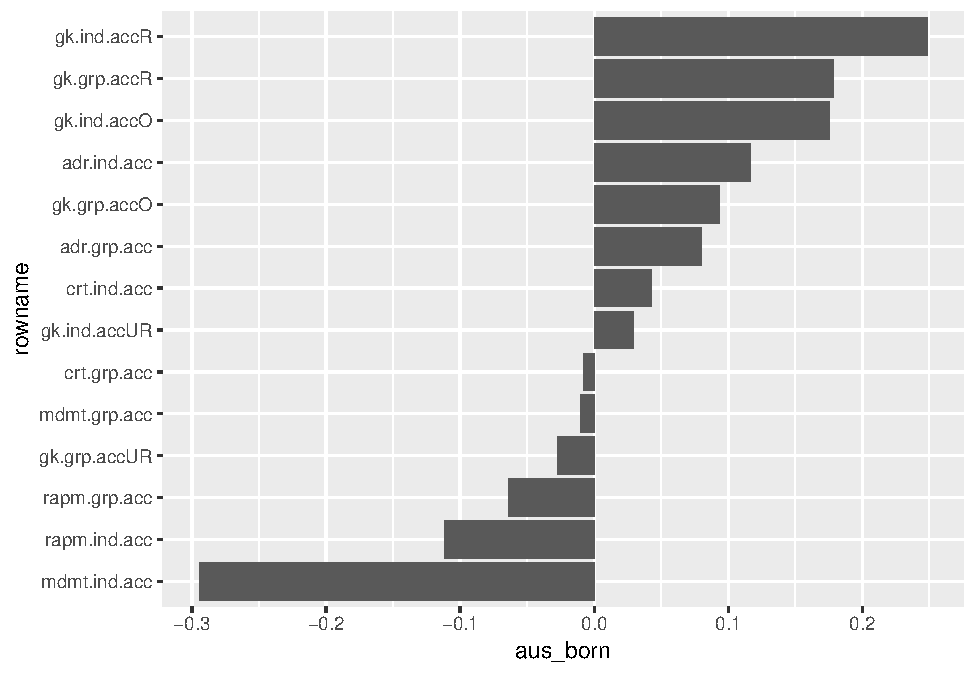
\includegraphics{corr_analyses_files/figure-latex/unnamed-chunk-1-3.pdf}
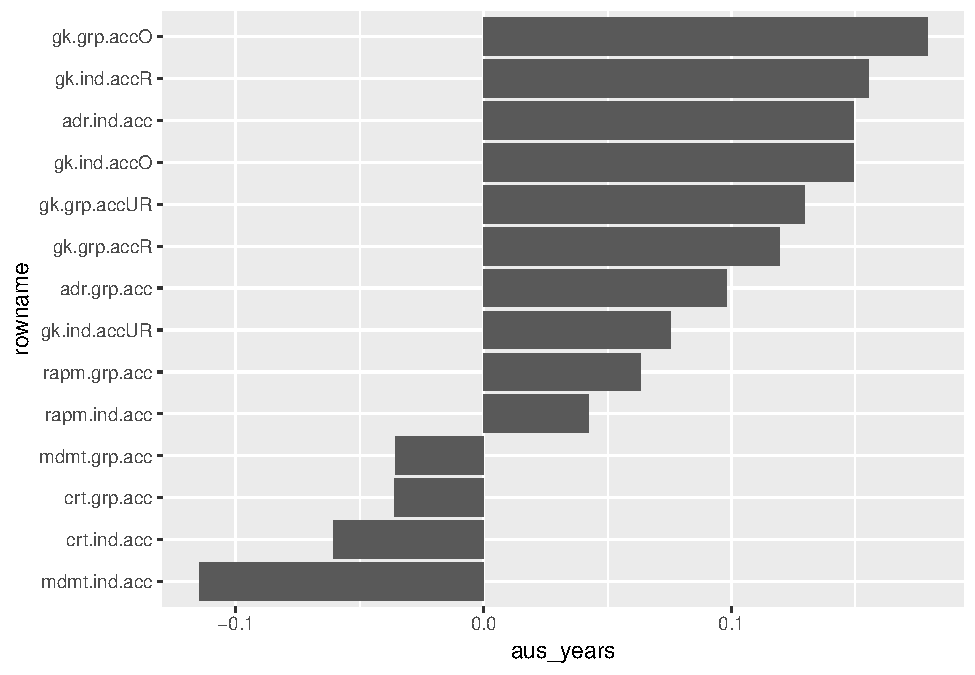
\includegraphics{corr_analyses_files/figure-latex/unnamed-chunk-1-4.pdf}
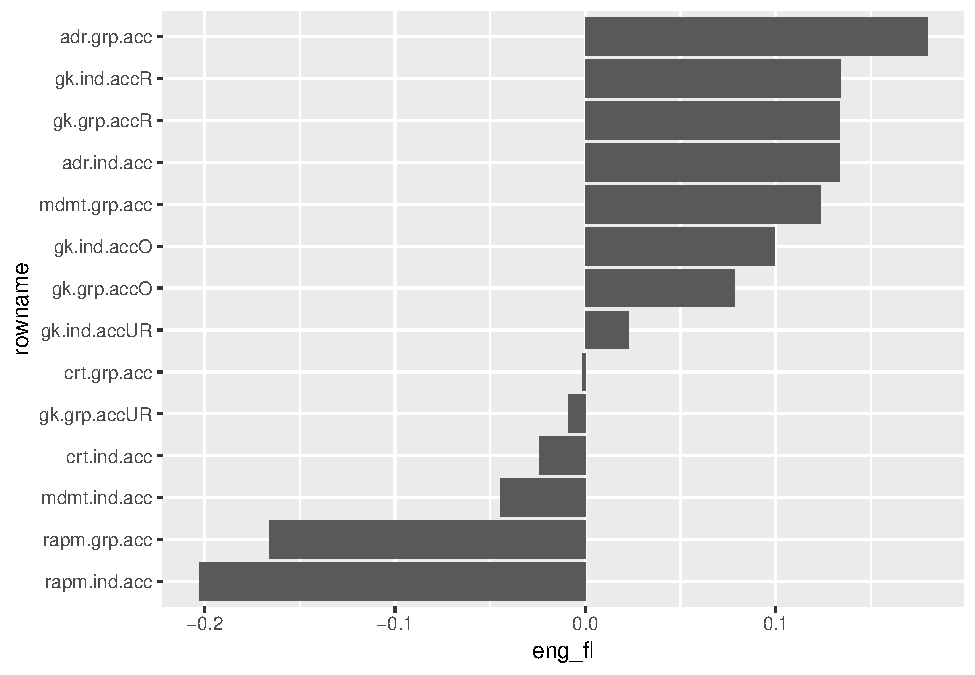
\includegraphics{corr_analyses_files/figure-latex/unnamed-chunk-1-5.pdf}
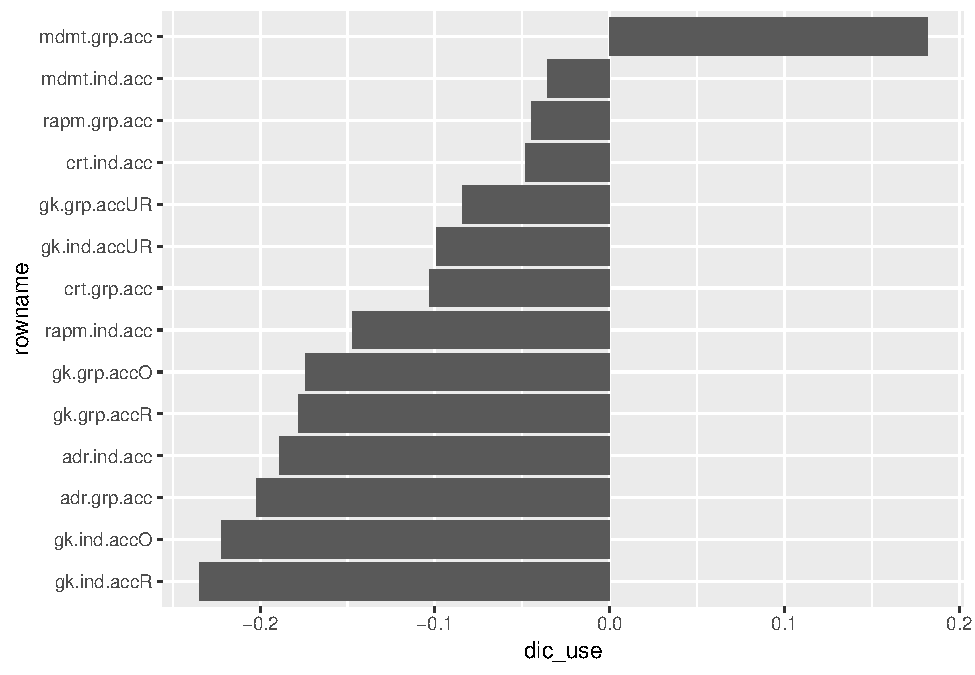
\includegraphics{corr_analyses_files/figure-latex/unnamed-chunk-1-6.pdf}


\end{document}
